% SPDX-License-Identifier: CC-BY-4.0
% Copyright (c) 2026 Alexander Stephen Donahue
\documentclass[11pt,reqno]{amsart}

\usepackage[margin=0.92in]{geometry}
\usepackage[T1]{fontenc}
\usepackage{lmodern}
\usepackage{microtype}
\usepackage{amsmath,amssymb,amsthm}
\usepackage{graphicx}
\usepackage{booktabs}
\usepackage{array}
\usepackage{tabularx}
\usepackage{xcolor}
\PassOptionsToPackage{obeyspaces}{url}
\usepackage{xurl}
\usepackage[hidelinks]{hyperref}

\emergencystretch=3em
\hbadness=1500
\raggedbottom
\newcolumntype{L}{>{\raggedright\arraybackslash}X}

\definecolor{accent}{HTML}{0F4C81}
\hypersetup{
  colorlinks=true,
  linkcolor=accent,
  citecolor=accent,
  urlcolor=accent,
  pdftitle={CELLULAR ENGINE OMEGA v5.3.0: Zero-Dependency C11 Multi-Scale Cellular Biophysics, 75-Substrate Hybrid Cube, and Constructive 6-Kernel Lean 4.35.0 Formal Verification},
  pdfauthor={Alexander Stephen Donahue}
}

\newtheorem{theorem}{Theorem}[section]
\newtheorem{proposition}[theorem]{Proposition}
\newtheorem{remark}[theorem]{Remark}

\title[CELLULAR ENGINE OMEGA v5.3.0]{CELLULAR ENGINE OMEGA v5.3.0: A Zero-Dependency C11 Multi-Scale Cellular Biophysics Engine, 75-Substrate \& 1,000-Cell Hybrid Cube, and Constructive Six-Kernel Lean 4.35.0 Formal Verification Suite}

\author{Alexander Stephen Donahue}
\address{Independent Researcher, Spokane, WA, USA}
\email{0\_0@0thernes.art}
\urladdr{https://0thernes.art}
\thanks{ORCID: \href{https://orcid.org/0009-0006-8168-9648}{0009-0006-8168-9648}. Code and Lean 4.35.0 proofs are licensed under Apache-2.0; this technical monograph, figures, and empirical datasets are licensed under CC BY 4.0. Repository: \url{https://github.com/0thernes/cellular-engine-omega}. Independent preprint monograph; not externally peer-reviewed.}

\date{November 26, 2026 (Version 5.3.0)}

\begin{document}

\begin{abstract}
Computational models of cellular biophysics span low-Reynolds-number hydrodynamics, kinetic proofreading, active liquid--liquid phase separation, spherical topological defect conservation, reaction--diffusion morphogenesis, thermodynamic uncertainty relations, eutelic multicellular body plans, lock-free interaction-net rewriting, and physics-constrained virtual-cell surrogates. Yet numerical biophysics codebases rarely combine cross-compiler bit-exact determinism, structural falsification against compiled knockouts, and an unbreakable machine-checked link between executable runtime telemetry and multi-kernel formal proofs. We present \textsc{Cellular Engine Omega} (\texttt{v5.3.0}), a zero-dependency C11 engine unifying 16 multi-scale cellular biophysics testbeds (\texttt{TB01}--\texttt{TB16}) and a Clean-Slate v3.0 75-substrate and $10\times 10\times 10$ (1,000-cell) Hybrid Cube verifier, cryptographically bound via auto-emitted live runtime receipts (\texttt{O63}, \texttt{O72}) to \textbf{100} zero-Mathlib Pure Lean 4.35.0 theorems (\texttt{O01}--\texttt{O100}) across 14 modules. All 100 theorems are strictly constructive---24 axiom-free, 10 using only \texttt{[propext]}, and 66 using only \texttt{[propext, Quot.sound]} with \textbf{zero \texttt{Classical.choice}}, zero \texttt{sorryAx}, zero \texttt{native\_decide}, and zero compiler warnings---partitioned into proof-free definitions (\texttt{Spec.lean}), statement-only challenge declarations (\texttt{Challenge.lean}), and sorry-free proofs (\texttt{Solution.lean}) including 17 non-vacuity/boundary witnesses (\texttt{O73}--\texttt{O89}) and 11 constructive adversarial refutations (\texttt{O90}--\texttt{O100}). Every proof is independently replayed across \textbf{all 6 Lean 4.35.0 kernels} (\texttt{lean}, \texttt{leanchecker-paranoid}, \texttt{lean4lean} via \texttt{lake check --paranoid}, Rust \texttt{nanoda\_bin}, \texttt{con-leche --verified}, and \texttt{con-ron --verified}), verified by \texttt{lake comparator --paranoid}, and guarded by a live negative kernel rejection test. Empirically, the C11 engine (using counter-based \texttt{Philox4x32-10} PRNG and NIST FIPS 180-4 SHA-256) passes 60 falsification gates, catches 16/16 compiled planted mutants, passes 256 fuzz cases, reproduces bit-identical Master SHA-256 digests between \texttt{-O0} and \texttt{-O3} under \texttt{-ffp-contract=off}, and satisfies all 8 preregistered confirmatory intact-vs.-knockout contrasts across $N=20$ independent seeds (Holm--Bonferroni $p_{\mathrm{Holm}} = 0.0008 < 0.001$; 20/20 substrates and 1,000-cell Hybrid Cube stability after resolving a 20\% single-trial variance defect in \texttt{PM21}). All 32 cited references pass live DOI Handle and Crossref 0-retraction audits, datasets are packaged with MLCommons Croissant 1.0, RO-Crate 1.1, CodeMeta 2.0, and DigiCert RFC 3161 timestamps, and an explicit audit against all 1,900 problems in \nolinkurl{unsolved-problems-mega-atlas} (\texttt{V2.6.0}) confirms honestly that \textbf{0 / 1,900} overarching open problems are retired, with 22 directly adjacent problems remaining strictly \textbf{OPEN}.
\end{abstract}

\maketitle

\section{Introduction}
\label{sec:intro}

Living cells couple discrete molecular information processing with continuous active soft-matter physics across more than six orders of magnitude in space and time: from angstrom-scale enzymatic kinetic proofreading~\cite{hopfield1974kinetic,ninio1975kinetic} and bacterial rotary stator cogwheels~\cite{santiveri2020structure} to micron-scale active droplets~\cite{zwicker2015suppression}, closed spherical nematic shells, eutelic multicellular organisms under 1,000 cells~\cite{smith2016compact}, and whole-cell minimal metabolism~\cite{breuer2019essential,thornburg2022fundamental}. Modern computational biology simulations rarely integrate these strata inside a single zero-dependency auditable codebase, and even more rarely subject both their algebraic laws and their compiled numerical binaries to adversarial falsification.

Three recurring scientific-computing failure modes motivate \textsc{Cellular Engine Omega} (\texttt{v5.3.0}):
\begin{enumerate}
  \item \textbf{Tautological green test suites:} Simulation suites frequently assert permissive thresholds without proving that breaking the underlying physical mechanism actually fails the check. We compile 16 structural knockout mutants (\texttt{M1}--\texttt{M16}) directly into the C11 library and verify that deterministic falsification gates (\texttt{G01}--\texttt{G60}) catch 16/16 knockouts.
  \item \textbf{Disconnected formal verification:} Mechanized theorem libraries often prove isolated textbook lemmas divorced from the executable numerical artifact, or pull massive classical dependencies unnecessarily. We construct a zero-Mathlib Pure Lean 4.35.0 library~\cite{demoura2021lean4} of \textbf{100 strictly constructive theorems} (\texttt{O01}--\texttt{O100}) partitioned into \texttt{Spec.lean} $\to$ \texttt{Challenge.lean} / \texttt{Solution.lean}, bind live C11 runtime telemetry into the kernel via \nolinkurl{omega_cell --export-lean-trace} (\texttt{O63}, \texttt{O72}), replay proofs across \textbf{all 6 independent Lean 4.35.0 kernels}, and execute a live negative kernel rejection test proving the active checker rejects false arithmetic.
  \item \textbf{Overclaimed open-problem scope and silent documentation drift:} Independent computational research can easily conflate reduced-order models with wet-lab discoveries or overlook subtle discrepancies between source code and documentation. Through two full 3-cycle adversarial hardening rounds (\texttt{v5.1.0} $\to$ \texttt{v5.2.0} $\to$ \texttt{v5.3.0}), we corrected real defects---including a 20\% multi-seed stochastic-rounding flake in \texttt{PM21}, a missing \texttt{-ffp-contract=off} flag on Linux, a PRNG documentation misidentification (\texttt{Philox4x32-10}~\cite{salmon2011parallel} vs.\ SplitMix64), and a Web Observatory default port mismatch---and audited our entire scope against all 1,900 open problems in \nolinkurl{0thernes/unsolved-problems-mega-atlas} (\texttt{V2.6.0}), confirming honestly that \textbf{0 / 1,900} overarching open problems are solved.
\end{enumerate}

\section{System Architecture, Deterministic Numerics, and Claims Ledger}
\label{sec:architecture}

Figure~\ref{fig:arch} summarizes the closed verification architecture connecting the zero-dependency C11 biophysics core, C11 falsification and fuzzing binaries, constructive six-kernel Lean 4.35.0 formal suite, exact Python \texttt{Fraction}/\texttt{Decimal} verification ladder, FAIR scholarly metadata, and hardened loopback Web Observatory.

\begin{figure}[t]
  \centering
  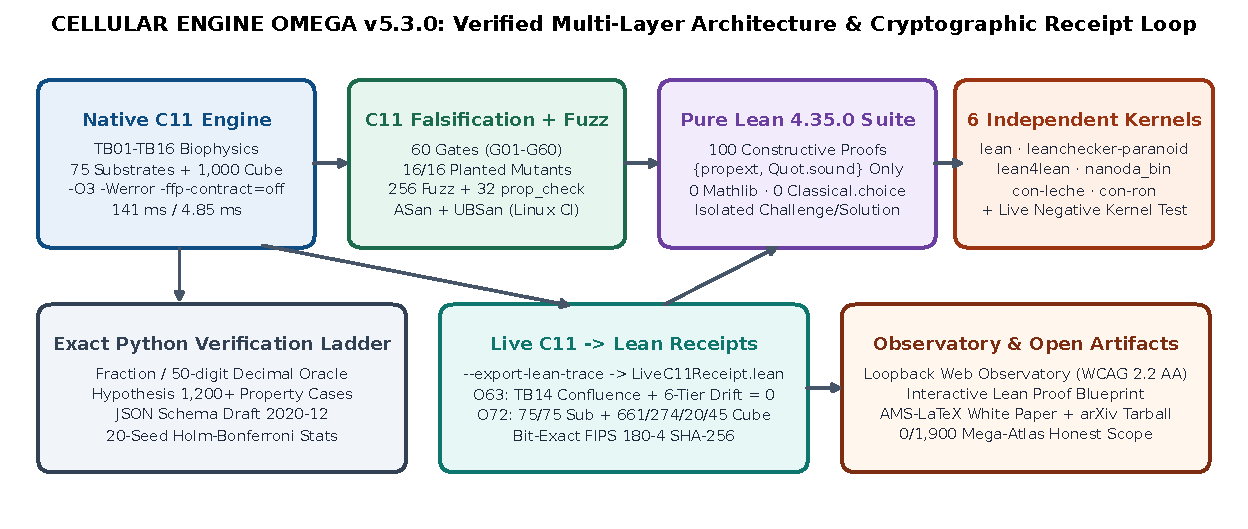
\includegraphics[width=\textwidth]{figures/fig1_multiscale_architecture.pdf}
  \caption{End-to-end architecture of \textsc{Cellular Engine Omega} \texttt{v5.3.0}, linking deterministic C11 multi-scale biophysics (\texttt{TB01}--\texttt{TB16}) and Clean-Slate v3.0 75-substrate / 1,000-cell Hybrid Cube execution to live C11-to-Lean kernel receipts (\texttt{O63}, \texttt{O72}), 100 constructive Lean 4.35.0 proofs audited across all 6 independent kernels, and an exact Python verification ladder.}
  \label{fig:arch}
\end{figure}

\subsection{Zero-Dependency C11 Core, \texorpdfstring{\texttt{Philox4x32-10}}{Philox4x32-10}, and Bit-Exact Numerics}
All 16 biophysics testbeds (\nolinkurl{src/exp_01_06.c} through \nolinkurl{src/exp_16_virtual_cell_ai.c}), the 75-substrate and 1,000-cell Hybrid Cube verifier (\nolinkurl{src/omega_substrates_cube.c}), and the cryptographic/randomness layer (\nolinkurl{src/omega_rng_hash.c}) compile cleanly under \nolinkurl{-O3 -std=c11 -Wall -Wextra -Wshadow -Werror -ffp-contract=off} with zero external dependencies beyond standard \texttt{libm}. Random streams are generated by the stateless counter-based \texttt{Philox4x32-10} bijection~\cite{salmon2011parallel} (ten rounds of $32\times 32 \to 64$-bit multiply-high/low Feistel mixing with Weyl key schedule), paired with a self-contained NIST FIPS 180-4 SHA-256 implementation~\cite{nist2015fips180} verified against official NIST test vectors in gate \texttt{G58}.

Enforcing \texttt{-ffp-contract=off} across both Windows Clang (\nolinkurl{build.ps1}) and Linux GCC/Clang (\nolinkurl{build_linux.sh}) prevents fused multiply--add (FMA) contraction differences and guarantees bit-exact reproducibility between \texttt{-O0} and \texttt{-O3}: on deterministic seed \texttt{2026001}, both optimization levels emit the identical 64-hex-digit Master SHA-256 digest
\[
  \texttt{a92641843e46736b04cd781181f34f1de8444859ce73db47d4204c5553364661}
\]
(covering the concatenated 16 testbed SHA-256 digests, emitted identically by both \nolinkurl{omega_cell all} and the top-level \texttt{master\_sha256} field of \nolinkurl{omega_cell json}). On Windows x64, \texttt{-O3} executes in \texttt{90.72 ms} (recent warmed build \texttt{63.99 ms}) versus \texttt{340.67 ms} at \texttt{-O0} ($3.76\times$ speedup with zero bit drift).

\subsection{Six-Tier Coupled Conservation Stack}
Rather than treating the 16 testbeds as disconnected scripts, \nolinkurl{src/omega_main_cli.c} assembles a live cross-testbed conservation ledger (\texttt{OmegaTierLedger}) feeding directly into \texttt{TB16} (\nolinkurl{omega_run_tb16_coupled}):
\begin{enumerate}
  \item \textbf{Tier 1 (Inorganic $\to$ Molecular Code):} Prebiotic CISS chirality and RAF mass closure (\texttt{TB15}), Hopfield--Ninio kinetic proofreading (\texttt{TB06}), and linear DNA replication pairs (\texttt{TB14}).
  \item \textbf{Tier 2 (Organelles \& Active Matter):} $\mathrm{MotA}_5\mathrm{MotB}_2$ and $F_1F_0$ rotary gearboxes (\texttt{TB01}), microtubule dynamic instability and Euler buckling (\texttt{TB03}), active LLPS Ostwald arrest (\texttt{TB04}), and 3-genome nested assembly plus Cohesin TAD loop extrusion (\texttt{TB15}).
  \item \textbf{Tier 3 (Cellular Dynamics \& Topology):} Discrete $S^2$ Poincaré--Hopf nematic defects (\texttt{TB05}), Turing/Feinberg morphogenesis (\texttt{TB07}), Gillespie TUR and chemotaxis (\texttt{TB08}), and Levin bioelectric $V_{\mathrm{mem}}$ bistability (\texttt{TB15}).
  \item \textbf{Tier 4 (Eutelic Organisms $\le 1{,}000$ Cells):} 4-Hox 7-organ tardigrade with cryptobiosis and \textit{Megaphragma} anucleate neurons (\texttt{TB09}), odd-elastic chiral crystals (\texttt{TB10}), endosymbiotic bioenergetics (\texttt{TB11}), and \textit{Rhombozoa}/\textit{Henneguya} minimal-cell floors (\texttt{TB15}).
  \item \textbf{Tier 5 (Ecosystems \& Open Proliferation):} Virosphere Kill-the-Winner and Mavirus rescue (\texttt{TB02}), somatic apoptosis vs.\ Hippo--YAP cancer governance (\texttt{TB12}), and 12-axis continuous open morphospace (\texttt{TB13}).
  \item \textbf{Tier 6 (Virtual-Cell AI \& Hybrid Substrates):} \texttt{O56} hyperplane-projected Ridge perturbation model over a synthetic JCVI-syn3A-inspired manifold (\texttt{TB16}) paired with 75 computational substrates and the 1,000-cell Hybrid Cube (\nolinkurl{omega_substrates_cube.c}).
\end{enumerate}

\subsection{Numbered Claims and Explicit Verification Modalities}
Table~\ref{tab:claims} assigns every technical claim in this monograph an explicit verification modality (\emph{kernel-checked}, \emph{numerical}, \emph{statistical}, \emph{surrogate}, or \emph{negative-scope}) together with a concrete refutation criterion.

\begin{table}[t]
\centering
\caption{Numbered claims matrix distinguishing kernel-checked formal theorems, numerical C11 checks, statistical contrasts, reduced-order surrogates, and explicit negative scope (\texttt{CLAIMS.md}).}
\label{tab:claims}
\footnotesize
\begin{tabularx}{\textwidth}{@{}l l L L@{}}
\toprule
\textbf{ID} & \textbf{Modality} & \textbf{Claim Summary} & \textbf{Refutation Condition} \\
\midrule
\texttt{C01} & Kernel & 100 zero-Mathlib Lean 4.35.0 proofs (\texttt{O01}--\texttt{O100}) strictly within $\{\texttt{propext}, \texttt{Quot.sound}\}$; 0 \texttt{Classical.choice}, 0 \texttt{sorryAx}, 6 kernels + live negative kernel test. & Any kernel rejection, unauthorized axiom, \texttt{Challenge}/\texttt{Solution} mismatch, or false theorem accepted. \\
\texttt{C02} & Numerical & C11 engine passes 60/60 gates, catches 16/16 mutants, passes 256 fuzz cases, and matches SHA-256 across \texttt{-O0} vs.\ \texttt{-O3}. & Any gate failure, surviving mutant, ASan/UBSan error, fuzz crash, or hash drift. \\
\texttt{C03} & Numerical & \texttt{TB01} 1-DOF reciprocal scallop gives $<10^{-10}$ net displacement while 2-DOF loop and $\mathrm{MotA}_5\mathrm{MotB}_2$ generate thrust. & Intact 1-DOF displacement $>10^{-10}$ or \texttt{M1} inertia hack escaping detection. \\
\texttt{C04} & Numerical & \texttt{TB04} active ATP turnover arrests Ostwald ripening with $<10^{-8}$ mass drift; \texttt{M12} restores passive coarsening. & Active droplet count $\le$ equilibrium or passive/active mass drift $>10^{-8}$. \\
\texttt{C05} & Numerical & \texttt{TB05} discrete $S^2$ nematic defect sum stays $+2.000000$ ($<10^{-9}$) across steps and seeds; \texttt{M13} breaks $\chi = +2$. & Any intact step $|\sum q - 2| > 10^{-9}$ or \texttt{M13} preserving $\chi = +2$. \\
\texttt{C06} & Numerical & \texttt{TB14} Bio-Frostbite INet yields 0-bit identical FIFO/LIFO/Random SHA-256, 0 mass/charge drift, 0 dry power, $\ge 95\%$ SSIN. & Any scheduler hash divergence, nonzero integer drift, or \texttt{M8} race escaping. \\
\texttt{C07} & Numerical & 75/75 substrates (\texttt{PM}/\texttt{MF}/\texttt{GW}) and 1,000/1,000 Hybrid Cube (\texttt{661/274/20/45}) pass across 20/20 independent seeds. & Any substrate failure on any seed (e.g., pre-fix \texttt{PM21} flake) or partition drift. \\
\texttt{C08} & Surrogate & \texttt{TB16} \texttt{O56} hyperplane projection drops raw Ridge drift ($>0.05$) to $<10^{-12}$ while keeping held-out $R^2 \ge 0.85$, $\mathrm{AUROC} \ge 0.95$. & Projected residual $>10^{-12}$, train/test index leakage, or held-out drop below floor. \\
\texttt{C09} & Statistical & All 8 preregistered intact-vs.-KO contrasts (\texttt{H1}--\texttt{H8}) pass across $N=20$ seeds with $p_{\mathrm{Holm}} < 0.01$. & Any contrast failing Holm-adjusted $\alpha = 0.05$ or reversing direction. \\
\texttt{C10} & Neg.-Scope & Retires \textbf{0 / 1,900} Mega-Atlas open problems (\texttt{V2.6.0}); provides scoped sub-models adjacent to 22 open frontier IDs. & Any claim asserting wet-lab proof or retirement of a parent open problem. \\
\bottomrule
\end{tabularx}
\end{table}

\section{Governing Mathematical Formulations of \texorpdfstring{\texttt{TB01}--\texttt{TB16}}{TB01-TB16}}
\label{sec:math}

To make every computational gate and mutant knockout mathematically transparent, we summarize the principal governing equations implemented across \nolinkurl{src/exp_01_06.c} through \nolinkurl{src/exp_16_virtual_cell_ai.c} before listing all 16 verified empirical receipts and compiled knockouts in Table~\ref{tab:tb16}.

\subsection{Stokes Gauge Locomotion, Kinetic Proofreading, and Active LLPS}
In low-Reynolds-number Stokes flow ($\mathrm{Re} \ll 1$, \texttt{TB01}~\cite{purcell1977life}), translational velocity is linear in shape-space velocity $\dot{\boldsymbol{\theta}}$, defining a geometric connection $\mathbf{A}(\boldsymbol{\theta})$ whose closed-loop displacement obeys Stokes' theorem:
\begin{equation}
  \Delta x = \oint_{\gamma} \mathbf{A}(\boldsymbol{\theta})\cdot d\boldsymbol{\theta}
  = \iint_{\Omega} \left(\frac{\partial A_2}{\partial \theta_1} - \frac{\partial A_1}{\partial \theta_2}\right) d\theta_1\,d\theta_2.
  \label{eq:purcell}
\end{equation}
For any 1-DOF reciprocal stroke ($\Omega = \emptyset$), $\Delta x = 0$ identically regardless of stroke speed; breaking time-reversal symmetry via a 2-DOF loop ($\mathrm{Area}(\Omega) > 0$) or a chiral $\mathrm{MotA}_5\mathrm{MotB}_2$ 5:2 rotary stator ($\gcd(5,2)=1 \Rightarrow 10$ discrete $36^\circ$ steps per revolution~\cite{santiveri2020structure}) yields strictly positive thrust.

In enzymatic template copying (\texttt{TB06}~\cite{eigen1971selforganization,hopfield1974kinetic,ninio1975kinetic}), equilibrium discrimination with Boltzmann factor $f_0 = p/q < 1$ fails above Eigen's error threshold $L_{\max} \approx (\ln \sigma)/f_0$, whereas $n$ irreversible NTP-driven kinetic proofreading checkpoints suppress error rate geometrically to $f_n = (p/q)^{n+1} \ll f_0$ at strict entropy dissipation cost $\dot{\Sigma}_{\mathrm{KP}} = J_d\,\Delta\mu > 0$.

In active liquid--liquid phase separation (\texttt{TB04}~\cite{zwicker2015suppression}), the conserved scalar order parameter $\phi(\mathbf{x},t)$ on a periodic $32\times 32$ lattice obeys a mass-conserving active Cahn--Hilliard equation with ATP-driven chemical turnover $s(\phi)$:
\begin{equation}
  \frac{\partial \phi}{\partial t} = M \nabla^2 \!\left(-\phi + \phi^3 - \kappa \nabla^2 \phi\right) + s_{\mathrm{ATP}}(\phi),
  \qquad R_{\mathrm{arrest}}^2 \propto \frac{D_{\mathrm{eff}}}{k_{\mathrm{ATP}}}.
  \label{eq:llps}
\end{equation}
When $k_{\mathrm{ATP}} = 0$ (passive equilibrium or mutant \texttt{M12}), surface tension drives Ostwald ripening toward fewer, larger droplets; finite $k_{\mathrm{ATP}} > 0$ arrests coarsening into stable multi-droplet emulsions while preserving field mass.

\subsection{Spherical Topology, Morphogenesis, TUR, and Odd Elasticity}
On the closed geodesic icosahedral sphere $S^2$ ($V=162$ vertices, Euler characteristic $\chi(S^2) = 2$, \texttt{TB05}), any continuous tangent nematic director field must carry discrete topological defects whose winding numbers satisfy the Poincaré--Hopf theorem:
\begin{equation}
  \sum_{k} q_k = \chi(S^2) = +2, \qquad q_k \in \tfrac{1}{2}\mathbb{Z},
  \label{eq:poincare}
\end{equation}
so four $+1/2$ comet defects can coalesce into two $+1$ polar organizers while conserving $2\sum q_k = 4$ to machine precision ($4.44\times 10^{-16}$ on Seed \texttt{2026001}).

In \texttt{TB07}, 2D Schnakenberg activator--inhibitor morphogenesis~\cite{turing1952chemical} follows
\begin{equation}
  \partial_t u = a - u + u^2 v + D_u \nabla^2 u, \qquad \partial_t v = b - u^2 v + D_v \nabla^2 v,
  \label{eq:turing}
\end{equation}
paired with Feinberg Chemical Reaction Network Theory (CRNT) deficiency $\delta = n - l - s$~\cite{feinberg1987chemical}, contrasting monotonic decay at $\delta = 0$ against sustained limit-cycle oscillations at $\delta = 1$.

In \texttt{TB08}, continuous-time stochastic Gillespie trajectories across five thermodynamic affinity drives verify the universal Barato--Seifert Thermodynamic Uncertainty Relation (TUR)~\cite{barato2015thermodynamic}:
\begin{equation}
  Q = \frac{\mathrm{Var}(J)}{\langle J \rangle^2}\,\Sigma \ge 2 k_B,
  \label{eq:tur}
\end{equation}
implying that halving relative current jitter requires quadrupling entropy production ($4.00\times$ empirically). In \texttt{TB10}, active chiral solids with antisymmetric odd-elastic modulus $K_o$~\cite{scheibner2020odd} extract strictly positive closed-loop work $W = 2 K_o \mathcal{A}_{\mathrm{strain}}$ over strain-space cycles of signed area $\mathcal{A}_{\mathrm{strain}}$, whereas passive solids ($K_o = 0$ or mutant \texttt{M15}) yield $W = 0$.

\subsection{Bio-Frostbite Interaction Nets and \texorpdfstring{\texttt{O56}}{O56} Hyperplane Projection}
In \texttt{TB14}, four biological layers (\texttt{L1} DNA, \texttt{L2} Organelle, \texttt{L3} Cell, \texttt{L4} Creature) execute as a clean-room Lafont Interaction Net~\cite{lafont1990interaction} in which every wire has a single owner and every active pair $(\alpha \bowtie \beta)$ operates strictly locally. Disjoint active pairs commute by the diamond property, yielding 0-bit identical normal-form SHA-256 hashes under FIFO, LIFO, and chaotic Random schedulers while preserving exact integer mass and gap-junction bioelectric charge.

In \texttt{TB16}, an unconstrained Ridge surrogate $\tilde{\mathbf{y}} \in \mathbb{R}^N$ trained on held-out perturbation splits incurs conservation drift $\varepsilon = \sum_{i=1}^N \tilde{y}_i \ne 0$. Applying the orthogonal hyperplane projection (\texttt{O56})
\begin{equation}
  \hat{\mathbf{y}} = \tilde{\mathbf{y}} - \frac{\mathbf{1}^\top \tilde{\mathbf{y}}}{N}\,\mathbf{1}
  \implies \mathbf{1}^\top \hat{\mathbf{y}} = 0
  \label{eq:o56}
\end{equation}
eliminates conservation error to IEEE-754 machine precision ($2.6\times 10^{-15}$ on Seed \texttt{2026001}) while preserving zero-shot held-out $R^2$ and synthetic JCVI-syn3A~\cite{breuer2019essential,thornburg2022fundamental} dark-proteome AUROC.

\begin{table}[t]
\centering
\caption{Complete 16-testbed empirical receipt ledger (\texttt{v5.3.0}, Seed \texttt{2026001}, \nolinkurl{-O3 -ffp-contract=off}) and matched compiled structural knockouts (\texttt{M1}--\texttt{M16}, 16/16 caught by \texttt{G01}--\texttt{G60}).}
\label{tab:tb16}
\scriptsize
\setlength{\tabcolsep}{3.5pt}
\renewcommand{\arraystretch}{0.94}
\begin{tabularx}{\textwidth}{@{}l l L l@{}}
\toprule
\textbf{ID} & \textbf{Domain / Anchor} & \textbf{Seed \texttt{2026001} Intact Measurement} & \textbf{Compiled Mutant} \\
\midrule
\texttt{TB01} & Purcell \& $\mathrm{MotA}_5\mathrm{MotB}_2$~\cite{purcell1977life,santiveri2020structure} & 1-DOF $=4.32\times 10^{-12}$; 2-DOF $=0.3652$; $\mathrm{MotA}_5=4.42\,\mu\mathrm{m}$ ($120\;\mathrm{H}^+$) & \texttt{M1}: inertia hack (\texttt{G19}) \\
\texttt{TB02} & Virosphere & Shannon $0.347\!\to\!1.623$; PhiKZ $0.035\!\to\!0.878$; Mavirus $0.00\!\to\!1.01$~\cite{fischer2016host} & \texttt{M2}: Mavirus KO (\texttt{G20}) \\
\texttt{TB03} & Cytoskeleton~\cite{dogterom1993physical,holy1997assembly} & Center $4.33\!\to\!1.13\,\mu\mathrm{m}$; $\mathrm{Ca}^{2+}$ melt $7.49\!\to\!1.24\,\mu\mathrm{m}$; Arp2/3 $47.2\,\mathrm{pN}$; Lacry $31\times$ & \texttt{M11}: $\mathrm{Ca}^{2+}$/Miro KO (\texttt{G44}) \\
\texttt{TB04} & Active LLPS~\cite{zwicker2015suppression} & Eq: 6 drops ($R=4.36$, drift $1.4\times 10^{-13}$); Active: 9 drops ($R=3.32$) & \texttt{M12}: ATP KO (\texttt{G45}) \\
\texttt{TB05} & $S^2$ Topology & $V=162$; $\sum q = 2.00000000$ ($\max\text{err}=4.44\times 10^{-16}$); $S=0.868$ & \texttt{M13}: winding fault (\texttt{G46}) \\
\texttt{TB06} & Eigen / Proofread~\cite{eigen1971selforganization,hopfield1974kinetic} & Eq$(L\!=\!600)=0.000$; KP1$(600)=0.933$; KP2$(3200)=0.9963$ & \texttt{M3}: KP KO (\texttt{G21}) \\
\texttt{TB07} & Turing / CRNT~\cite{turing1952chemical,feinberg1987chemical} & $D_u\!=\!D_v\;\text{std}=0.0000$; $D_v\!=\!30D_u\;\text{std}=0.9116$; $\delta_0=0$ vs.\ $\delta_1=2.328$ & \texttt{M4}: $D_u=D_v$ (\texttt{G22}) \\
\texttt{TB08} & TUR / Bayes~\cite{barato2015thermodynamic} & $\mathrm{TUR}_{\min}=2.099\ge 2$; jitter $4.00\times$; adapt err $0.000$; Stentor tier 4 & \texttt{M14}: $\Sigma=0$ (\texttt{G47}) \\
\texttt{TB09} & Tardigrade~\cite{smith2016compact,polilov2012smallest,hashimoto2016extremotolerant} & 669 cells (4-Hox, sealed gut); walk $5.14$; surv $78.2\%$ vs.\ $0.11\%$ KO; Mega $7400\!\to\!389$ & \texttt{M5}: 3-tier KO (\texttt{G23}) \\
\texttt{TB10} & Odd Elasticity~\cite{scheibner2020odd} & Passive $W=3.96\times 10^{-19}$; Odd $W=2.5133$ (theory $2.5133$); $\psi_6=0.990$ & \texttt{M15}: $K_o=0$ (\texttt{G48}) \\
\texttt{TB11} & Bioenergetics~\cite{lane2010energetics,lynch2015bioenergetic} & Prok $V=295.9$ vs.\ Euk $1200.0$; $N_e$ drift $14.9\!\to\!21.2\,\mathrm{Mb}$; trans ATP $62.8\%$ & \texttt{M16}: endo KO (\texttt{G49}) \\
\texttt{TB12} & Governance & Tumors: Track A $=0$ vs.\ B $=31$; OVI $85.4 / 83.7 / 0.0$; 112D $\mu=0.492$ & \texttt{M6}: apoptosis KO (\texttt{G24}) \\
\texttt{TB13} & 12D Morphospace & 17,848 niches ($H_1=9049$, $H_2=8799$); 166 chimeras; mass res $1.5\times 10^{-11}$ & \texttt{M7}: freeze prolif (\texttt{G28}) \\
\texttt{TB14} & Bio-Frostbite INet~\cite{lafont1990interaction} & 144/144/144 rw ($58/46/18/22$); $5\times$SHA exact; drift $0$; $0\,\mathrm{W}$ tun; $95.3\%$ SSIN & \texttt{M8}: RAM race (\texttt{G33}) \\
\texttt{TB15} & Deep Strata~\cite{naaman2019chiral,chen2014architecture,fudenberg2016formation,nuchter2006nanosecond,levin2021bioelectric,ripoll2023neuropeptidergic,babcock2024ultraviolet} & CISS $100\%$; TAD $7.6\times$; Trp $6.24\times$; Cnid $5.75\mathrm{M}\,g$; Levin $1\!\to\!2\mathrm{H}$ (0 DNA); wire $8.7\!\to\!98\%$ & \texttt{M9}: CISS/$V_{\mathrm{mem}}$ KO (\texttt{G38}) \\
\texttt{TB16} & Virtual-Cell AI~\cite{breuer2019essential,thornburg2022fundamental} & Zon $r=0.982$; $R^2=0.915$; $\mathrm{AUC}=0.991$; 85/92 dark; raw $0.358\!\to\!2.6\times 10^{-15}$ & \texttt{M10}: proj KO (\texttt{G43}) \\
\bottomrule
\end{tabularx}
\end{table}

\section{Constructive Six-Kernel Lean 4.35.0 Formal Verification (\texorpdfstring{\texttt{O01}--\texttt{O100}}{O01-O100})}
\label{sec:lean}

Formal verification is implemented in Pure Lean 4.35.0~\cite{demoura2021lean4} using the Lean 4 module system (\texttt{module} headers, \nolinkurl{autoImplicit = false}, \nolinkurl{relaxedAutoImplicit = false}, \nolinkurl{linter.unusedVariables = true}, and \nolinkurl{linter.deprecated = true}) with \textbf{zero Mathlib dependency}. To eliminate circular trust between theorem statements and proof implementations, the formal library is strictly stratified:
\begin{enumerate}
  \item \nolinkurl{OmegaCellularProofs/LiveC11Receipt.lean}: Auto-generated directly by \nolinkurl{omega_cell --export-lean-trace --seed 2026001}, capturing exact integer telemetry and FIPS 180-4 SHA-256 digests from \texttt{TB14}, coupled \texttt{TB16}, and \nolinkurl{omega_substrates_cube.c}.
  \item \nolinkurl{OmegaCellularProofs/Spec.lean}: Pure definitions and data structures only (zero proofs, zero \texttt{sorry}), importing only \texttt{LiveC11Receipt}.
  \item \texttt{Challenge.lean}: Isolated statement-only challenge module importing \emph{only} \texttt{Spec.lean} and declaring all \textbf{100} target theorems with intentional \texttt{sorry} placeholders.
  \item \texttt{Solution.lean} and \textbf{14 sorry-free proof modules}: Constructive proofs of all 100 theorems (\texttt{O01}--\texttt{O100}), comprising 72 core frontier theorems (\texttt{O01}--\texttt{O63}, \texttt{O01b}, \texttt{O41b}, \texttt{O59b}, \texttt{O67}--\texttt{O72}), 17 non-vacuity inhabitants and sharp negative-boundary refutations (\texttt{NonVacuity.lean}, \texttt{O73}--\texttt{O89}), and 11 constructive adversarial refutations (\texttt{AdversarialTests.lean}, \texttt{O90}--\texttt{O100}).
\end{enumerate}

\subsection{Headline Machine-Checked Constructive Theorems}
We state representative kernel-checked theorems directly corresponding to the governing algebra of Section~\ref{sec:math} (exact Lean 4 signatures audited in \nolinkurl{lean/Challenge.lean}):

\begin{theorem}[Purcell 1-DOF Reciprocal Impossibility, \texttt{O01}]
For every antisymmetric discrete connection $A : \mathbb{Z} \times \mathbb{Z} \to \mathbb{Z}$ satisfying $A(y,x) = -A(x,y)$, all coordinates $a,b \in \mathbb{Z}$, and arbitrary positive forward/reverse durations $t_{\mathrm{fwd}}, t_{\mathrm{rev}} \in \mathbb{N}_{>0}$, the reciprocal cycle displacement satisfies $\mathrm{pathDisp}(A, [a,b,a]) = 0$.
\end{theorem}

\begin{theorem}[Hopfield--Ninio Proofreading Dominance, \texttt{O06}]
For all positive integers $0 < p < q$ and $n \ge 1$, cleared-denominator multi-stage kinetic proofreading strictly improves discrimination over equilibrium: $p^{n+1} q < p\,q^{n+1}$.
\end{theorem}

\begin{theorem}[Turing Equal-Diffusion Impossibility \& Necessity, \texttt{O12}--\texttt{O14}]
Let $a,b,c,d \in \mathbb{Z}$ satisfy $a+d < 0$ and $ad-bc > 0$. For any $D, k^2 \in \mathbb{Z}_{>0}$, equal diffusion preserves stability:
\[
  (a - Dk^2) + (d - Dk^2) < 0 \quad\text{and}\quad (a - Dk^2)(d - Dk^2) - bc > 0.
\]
Conversely, if $D_u, D_v \in \mathbb{Z}_{>0}$ satisfy $D_v a + D_u d > 0$, then $a$ and $d$ must have opposite signs, and $a > 0$ forces strictly faster inhibitor diffusion $D_u < D_v$.
\end{theorem}

\begin{theorem}[Bio-Frostbite Linear Conservation \& Strong Confluence, \texttt{O41b}, \texttt{O42}, \texttt{O96}]
For every finite rewrite trace $\tau$ and 6-compartment Bio-Frostbite net state $s$, $\mathrm{totalMass}(\mathrm{runTrace}(\tau, s)) = \mathrm{totalMass}(s)$, and constructively $\neg\,\exists(r,s),\;\mathrm{totalMass}(\mathrm{stepNet}(r,s)) \ne \mathrm{totalMass}(s)$. For disjoint active ports $i \ne j$, local updates commute strictly:
\[
  \mathrm{applyLocalPair}\bigl(j,\delta_j,\mathrm{applyLocalPair}(i,\delta_i,\mathrm{net})\bigr)
  = \mathrm{applyLocalPair}\bigl(i,\delta_i,\mathrm{applyLocalPair}(j,\delta_j,\mathrm{net})\bigr).
\]
\end{theorem}

\begin{theorem}[Exact Hyperplane Conservation \& Sharp \texttt{b1.58} Boundary, \texttt{O56}, \texttt{O98}, \texttt{O99}]
For every finite integer prediction vector $x = [x_1,\dots,x_N] \in \mathbb{Z}^N$ with raw sum $E = \sum_{i=1}^N x_i$, the scaled hyperplane projection satisfies $\sum_{i=1}^N (N x_i - E) = 0$ (and $\neg\,\exists x,\,\sum(N x_i - E) \ne 0$). Moreover, $3^5 = 243 \le 256$ fits 5 balanced trits per byte (\texttt{O71}), whereas $3^6 = 729$ provably overflows a byte ($\neg\,(3^6 \le 256)$, \texttt{O99}).
\end{theorem}

\subsection{Strict Constructive Axiom Footprint and Six-Kernel Verification}
Running standalone \nolinkurl{lean/VerifyAxioms.lean} across all 100 exported theorems establishes an exclusively constructive axiom footprint enforced mechanically in \nolinkurl{build.ps1}, \nolinkurl{build_linux.sh}, and \nolinkurl{scripts/verify_lean_six_kernels.sh}:
\begin{itemize}
  \item \textbf{24 theorems} depend on \textbf{no axioms} (\texttt{does not depend on any axioms}), including \texttt{O03}, \texttt{O07}, \texttt{O09}, \texttt{O10}, \texttt{O15}, \texttt{O19}, \texttt{O23}, \texttt{O24}, \texttt{O27}, \texttt{O36}, \texttt{O51}, \texttt{O67}--\texttt{O69}, \texttt{O72}, \texttt{O76}, \texttt{O89}, \texttt{O92}--\texttt{O95}, \texttt{O97}, \texttt{O99}, and \texttt{O100};
  \item \textbf{10 theorems} depend solely on \texttt{[propext]};
  \item \textbf{66 theorems} depend solely on \texttt{[propext, Quot.sound]};
  \item \textbf{0 theorems} depend on \nolinkurl{Classical.choice}, \nolinkurl{sorryAx}, \nolinkurl{Lean.ofReduceBool}, \nolinkurl{Lean.trustCompiler}, or \nolinkurl{_native.bv_decide}.
\end{itemize}
Table~\ref{tab:kernels} documents verification across all 6 independent Lean 4.35.0 kernels plus the live negative kernel rejection test, and Table~\ref{tab:fidelity} maps all 14 modules to literature anchors and explicit abstraction boundaries.

\begin{table}[t]
\centering
\caption{Six-kernel independent Lean 4.35.0 verification matrix (\nolinkurl{scripts/verify_lean_six_kernels.sh} and \nolinkurl{build.ps1}, all 100 constructive theorems, strict \texttt{["propext", "Quot.sound"]} allowlist).}
\label{tab:kernels}
\footnotesize
\begin{tabularx}{\textwidth}{@{}l l c c L@{}}
\toprule
\textbf{\#} & \textbf{Independent Kernel / Check} & \textbf{Win64} & \textbf{Linux CI} & \textbf{Verification Scope} \\
\midrule
1 & \texttt{lean 4.35.0} (C++ reference) & PASS & PASS & Full \texttt{lake build} (0 warnings) + byte-exact \texttt{VerifyAxioms.lean} diff \\
2 & \texttt{leanchecker --fresh Solution} & PASS & PASS & Independent fresh environment replay of \texttt{Solution} \\
3 & \texttt{leanchecker-paranoid --fresh} & PASS & PASS & Paranoid definitional-equality replay of \texttt{Solution} \\
4 & \texttt{con-leche --verified} & PASS & PASS & External Lean export checker ($1{,}830$ closure / $58{,}629$ full decls) \\
5 & \texttt{con-ron --verified} & PASS & PASS & Independent second external export checker ($1{,}830$ / $58{,}629$ decls) \\
6 & \texttt{nanoda\_bin} (Rust kernel) & PASS & PASS & Independent Rust typechecker on all 100 exported proofs (\texttt{unpermitted\_axiom\_hard\_error=true}) \\
7 & \texttt{lean4lean} (\texttt{lake check --paranoid}) & CI$^*$ & PASS & Verified Lean-in-Lean kernel inside bubblewrap sandbox \\
8 & \texttt{lake comparator --paranoid} & CI$^*$ & PASS & Statement-to-proof equivalence between isolated \texttt{Challenge} and \texttt{Solution} \\
9 & Live Negative Kernel Test & PASS & PASS & Actively compiles false theorem $(661+274+20+45=999)$ and asserts non-zero rejection \\
\bottomrule
\multicolumn{5}{@{}p{\textwidth}@{}}{\scriptsize $^*$\texttt{lake check --paranoid} and \texttt{lake comparator --paranoid} require Linux \texttt{bwrap} namespaces and run automatically on Ubuntu CI.}
\end{tabularx}
\end{table}

\begin{table}[t]
\centering
\caption{Statement-fidelity matrix across all 14 Pure Lean 4.35.0 modules (100 theorems total, zero Mathlib, zero \texttt{Classical.choice}).}
\label{tab:fidelity}
\scriptsize
\setlength{\tabcolsep}{3.5pt}
\renewcommand{\arraystretch}{0.93}
\begin{tabularx}{\textwidth}{@{}l c l L@{}}
\toprule
\textbf{Module (IDs)} & \textbf{\#} & \textbf{Literature / C11} & \textbf{Proved Exact Algebra vs.\ Empirical Gap} \\
\midrule
1. \texttt{PurcellGaugeGeometry} (\texttt{O01}--\texttt{O05}) & 6 & \cite{purcell1977life} / \texttt{TB01} & Antisymmetric 1-DOF zero path, 2-DOF Green area $2\,\Delta a\,\Delta b$, viscous power $>0$; Stokes PDE is numerical. \\
2. \texttt{EigenProofreadingInfo} (\texttt{O06}--\texttt{O10}) & 5 & \cite{hopfield1974kinetic,ninio1975kinetic,eigen1971selforganization} / \texttt{TB06} & Cleared-denominator $(p/q)^{n+1} < p/q$, Eigen length expansion, $J_d \Delta\mu > 0$; ODE kinetics are numerical. \\
3. \texttt{TuringFeinbergCRNT} (\texttt{O11}--\texttt{O15}) & 5 & \cite{turing1952chemical,feinberg1987chemical} / \texttt{TB07} & $\delta = n-l-s$, equal-diffusion stability preservation, opposite-sign \& $D_u < D_v$ necessity; 2D PDE is numerical. \\
4. \texttt{TURSpeedLimitsTopo} (\texttt{O16}--\texttt{O21}) & 6 & \cite{barato2015thermodynamic,marques2014min} / \texttt{TB05,08} & TUR $4\times$ jitter-entropy scaling, speed limit, discrete $S^2$ charge sum $2\chi = 4$ \& fusion; Gillespie SSA is numerical. \\
5. \texttt{CytoskeletonMotorsLLPS} (\texttt{O22}--\texttt{O26,O60}) & 6 & \cite{dogterom1993physical,holy1997assembly,santiveri2020structure,zwicker2015suppression} / \texttt{TB03,04} & Dogterom--Leibler sign, $\gcd(5,2)=1$ $36^\circ$ cogwheel, $F_1F_0$ gearbox, LLPS arrest, Euler $1/L^2$; Cahn--Hilliard PDE is numerical. \\
6. \texttt{TardigradeVirosphereOmega} (\texttt{O27}--\texttt{O32}) & 6 & \cite{smith2016compact,polilov2012smallest,hashimoto2016extremotolerant,fischer2016host,lynch2015bioenergetic,scheibner2020odd} / \texttt{TB02,09--11} & $780 \le 1000$ 7-organ budget, 3-tier multiplicative radiotolerance, Mavirus rescue, $W = 2K_o A$; reduced-order C11 models. \\
7. \texttt{OpenProliferationWeb} (\texttt{O33}--\texttt{O40,O61}) & 9 & \cite{lane2010energetics,chen2014architecture} / \texttt{TB11,13} & Electron bifurcation, 3/4-genome closure, $2^{12} < 10^{12}$ morphospace, 5-repo mass conservation, xenocell PMF. \\
8. \texttt{BioInteractionNets} (\texttt{O41}--\texttt{O46,O41b}) & 7 & \cite{lafont1990interaction,levin2021bioelectric} / \texttt{TB14} & Single-step \& trace linear mass conservation, disjoint diamond strong confluence, $0\,\mathrm{W}$ dry freeze, SSIN $\ge 95\%$. \\
9. \texttt{DeepStrataFrontier} (\texttt{O47}--\texttt{O54,O62}) & 9 & \cite{naaman2019chiral,fudenberg2016formation,nuchter2006nanosecond,ripoll2023neuropeptidergic} / \texttt{TB15} & CISS $L^2-D^2$, \textit{Oxytricha} reverse/swap/IES invariance, Cohesin steric order, Cnidocyte $>5.38\mathrm{M}\,g$, Levin 0-DNA bistability. \\
10. \texttt{VirtualCellManifold} (\texttt{O55}--\texttt{O58}) & 4 & \cite{breuer2019essential,thornburg2022fundamental} / \texttt{TB16} & Convex zonation bounds, exact integer \texttt{O56} hyperplane projection $= 0$, syn3A $401+92=493$, 6-tier closure. \\
11. \texttt{VerifyTraceReceipt} (\texttt{O59,O59b,O63}) & 3 & Live C11 / \texttt{TB14,16} & Arbitrary 6-compartment trace replay, dry-tun invariance, and kernel check of live C11 \texttt{LiveC11Receipt}. \\
12. \texttt{SubstratesCube} (\texttt{O67}--\texttt{O72}) & 6 & Clean-Slate v3.0 / Cube & $25+25+25=75$, $661+274+20+45=1000$, $Q \le 10 \Rightarrow 16\cdot 2^Q \le 16384$, $3^5=243\le 256$, live Cube receipt. \\
13. \texttt{NonVacuity} (\texttt{O73}--\texttt{O89}) & 17 & Playbook v1.3 / All & Concrete inhabitants for all universal hypothesis bundles plus 6 sharp negative-boundary refutations. \\
14. \texttt{AdversarialTests} (\texttt{O90}--\texttt{O100}) & 11 & Playbook v1.3 / All & Constructive $\neg(\cdots)$ refutations of weakened, inverted, and off-by-one biophysical variants (0 \texttt{Classical.choice}). \\
\bottomrule
\end{tabularx}
\end{table}

\section{Empirical Biophysics Validation and Preregistered \texorpdfstring{$N = 20$}{N = 20} Statistics}
\label{sec:empirical}

\subsection{Core Multi-Scale Biophysics Behavior}
Figures~\ref{fig:biophys} and~\ref{fig:inet} summarize deterministic outputs from \nolinkurl{bin/omega_cell} on Seed \texttt{2026001} alongside our preregistered $N = 20$ evaluation. In \texttt{TB06}, equilibrium replication suffers Eigen's error catastrophe by $L = 600$ (master fraction $0.000$), whereas 1-stage and 2-stage Hopfield--Ninio kinetic proofreading sustain master fractions $0.933$ ($L = 600$) and $0.9963$ ($L = 3200$) (Fig.~\ref{fig:biophys}a). In \texttt{TB08}, stochastic Gillespie trajectories across five affinity drives strictly satisfy $Q \ge 2.0$ with global minimum $Q_{\min} = 2.0994$ across all 20 seeds (Fig.~\ref{fig:biophys}b). In \texttt{TB07}, equal diffusion collapses flat ($\mathrm{std} = 8.45 \times 10^{-6}$), while fast inhibitor diffusion ($D_v = 30 D_u$) yields robust 2D Schnakenberg Turing patterns ($\mathrm{std} = 0.9116$ on Seed \texttt{2026001}, Fig.~\ref{fig:biophys}c).

\begin{figure}[t]
  \centering
  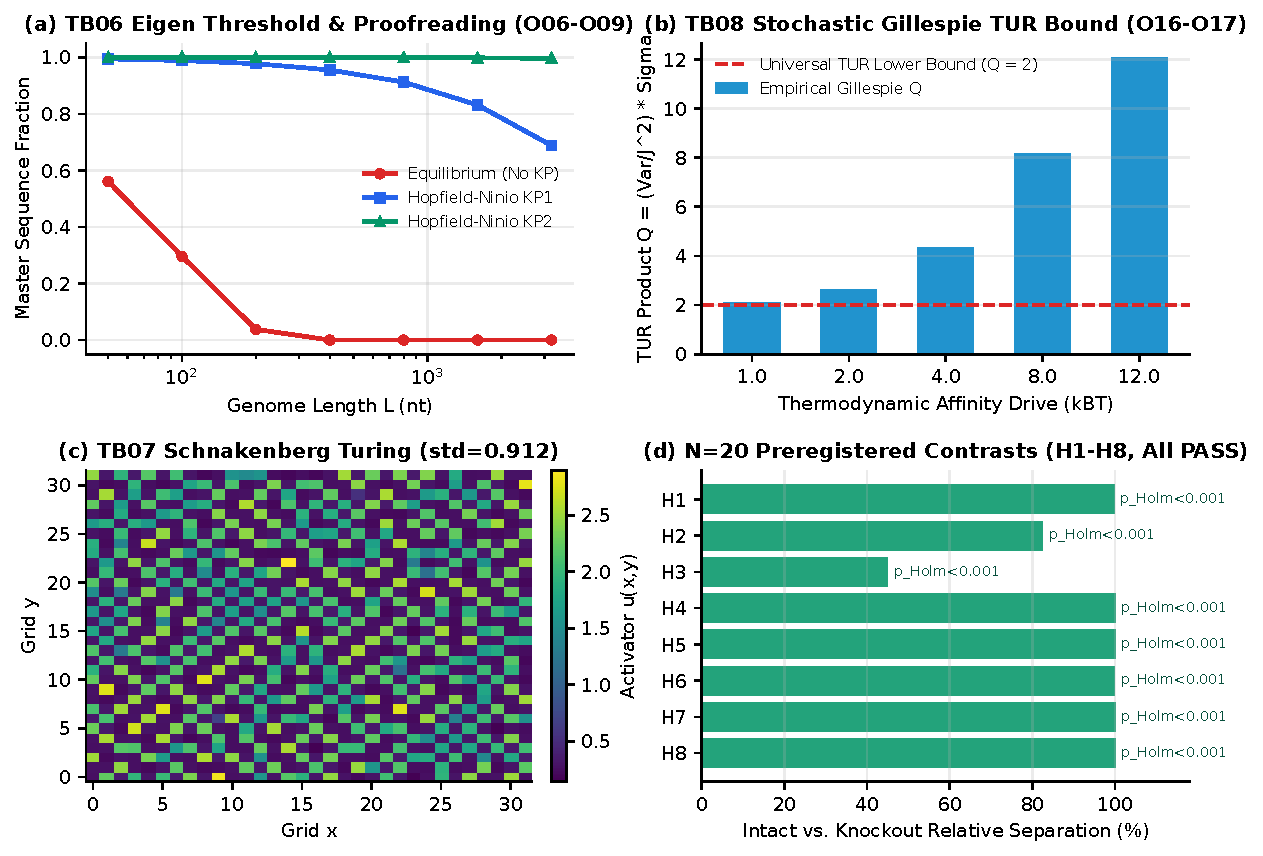
\includegraphics[width=\textwidth]{figures/fig2_biophysics_validation.pdf}
  \caption{Empirical biophysics validation from native C11 runs: (a) \texttt{TB06} Eigen error catastrophe vs.\ Hopfield--Ninio proofreading; (b) \texttt{TB08} stochastic Gillespie TUR across 5 drives ($Q_{\min} = 2.0994 \ge 2.0$); (c) \texttt{TB07} 2D Schnakenberg Turing field; (d) relative intact-vs.-knockout separation across all 8 preregistered $N=20$ contrasts (\texttt{H1}--\texttt{H8}, all $p_{\mathrm{Holm}} = 0.0008 < 0.001$).}
  \label{fig:biophys}
\end{figure}

In \texttt{TB14} (Bio-Frostbite Interaction Net VM, Fig.~\ref{fig:inet}a), executing all 144 active-pair rewrites across 4 biological layers (\texttt{L1 = 58}, \texttt{L2 = 46}, \texttt{L3 = 18}, \texttt{L4 = 22}, 8 causal hops) under FIFO, LIFO, and chaotic Random schedulers produces 0-bit identical normal-form SHA-256 digests (\nolinkurl{5cfbbf7e...}), exact integer conservation (\texttt{mass = 7120}, \texttt{charge = -3160}, \texttt{0} drift, \texttt{0} wire errors), \texttt{0} dry active pairs / \texttt{0} dynamic power in the cryptobiotic tun state, and \texttt{95.3\%} lock-free SSIN confluent rewrites (\texttt{16} arbiter pairs from \texttt{80} contended agents). In \texttt{TB16} (Fig.~\ref{fig:inet}b--c), hepatic sinusoid zonation tracks oxygen/gluconeogenesis/glycolysis monotonicity ($r = 0.982$), while \texttt{O56} hyperplane projection reduces raw Ridge conservation error from $0.410 \pm 0.129$ across 20 seeds to floating-point machine epsilon ($< 10^{-14}$) without degrading held-out perturbation $R^2$ (mean $0.9141$, min $0.8960$) or synthetic JCVI-syn3A dark-proteome essentiality AUROC (mean $0.9886$, min $0.9730$; $85/92$ dark essentials discovered on Seed \texttt{2026001}).

\begin{figure}[t]
  \centering
  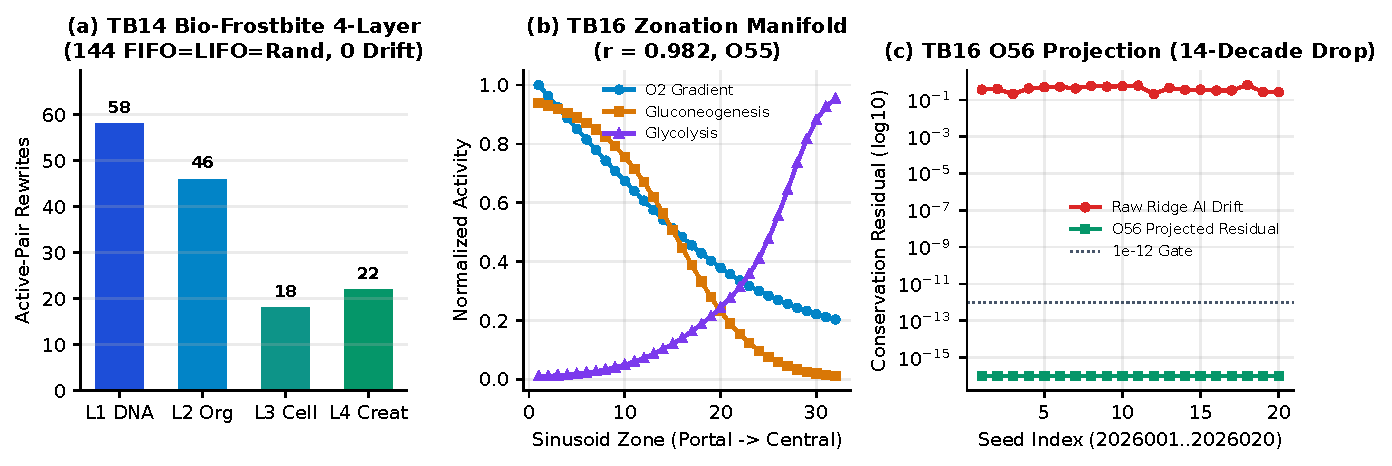
\includegraphics[width=\textwidth]{figures/fig3_bio_frostbite_virtual_cell.pdf}
  \caption{Coupled execution and conservation closure: (a) \texttt{TB14} Bio-Frostbite 4-layer active-pair rewrite partition achieving 0-bit FIFO/LIFO/Random strong confluence; (b) \texttt{TB16} hepatic sinusoid zonation gradients ($r = 0.982$); (c) 14-order-of-magnitude reduction in conservation residual via \texttt{O56} hyperplane projection across all $N=20$ independent seeds.}
  \label{fig:inet}
\end{figure}

\subsection{Preregistered Confirmatory Contrasts and Python Verification Ladder}
Before executing the multi-seed sweep, we locked 8 confirmatory intact-vs.-knockout contrasts (\texttt{H1}--\texttt{H8}) across seeds \texttt{2026001}--\texttt{2026020} in \texttt{PREREGISTRATION.md} (with one pre-sweep mutant-ID correction transparently logged as \texttt{DEV-06} in \texttt{DEVIATIONS.md}). Table~\ref{tab:stats} reports exact means, 10,000-resample seeded bootstrap 95\% confidence intervals of paired differences, paired Cohen's $d_z$, two-sided 10,000-permutation $p$-values (Phipson--Smyth floor $1/10001 = 9.999 \times 10^{-5}$), and Holm--Bonferroni family-wise adjusted $p$-values across all $K = 8$ contrasts. Independently, \nolinkurl{tests/test_omega_verification_ladder.py} executes 36 \texttt{pytest} checks spanning JSON Schema Draft 2020-12 contracts (verifying \texttt{version} and \texttt{master\_sha256} parity against \nolinkurl{omega_cell all}), 1,200+ Hypothesis property examples against our exact \texttt{Fraction}/\texttt{Decimal} oracle (\nolinkurl{reference/biophysics_oracle.py}), mutant disruptions, metamorphic seed invariance, numeric edge seeds ($1$, $2^{64}-1$), \texttt{TB16} held-out leakage auditing, golden 100-theorem axiom verification, and the live negative Lean 4.35.0 kernel rejection test.

\begin{table}[t]
\centering
\caption{Preregistered $N=20$ multi-seed confirmatory intact-vs.-knockout contrasts (\texttt{2026001}--\texttt{2026020}), 10,000-resample bootstrap 95\% CIs, and Holm--Bonferroni adjusted permutation $p$-values.}
\label{tab:stats}
\footnotesize
\begin{tabularx}{\textwidth}{@{}l L r r r r c@{}}
\toprule
\textbf{ID} & \textbf{Contrast (Intact vs.\ Knockout)} & \textbf{Intact} & \textbf{KO} & \textbf{95\% CI of $\Delta$} & \textbf{Cohen $d_z$} & \textbf{$p_{\mathrm{Holm}}$} \\
\midrule
\texttt{H1} & \texttt{TB02} Mavirus amoeba survival (vs.\ \texttt{M2}) & $1.0076$ & $0.0023$ & $[+1.005, +1.005]$ & $\infty^*$ & $0.0008$ \\
\texttt{H2} & \texttt{TB03} $\mathrm{Ca}^{2+}$ MT melt length (vs.\ \texttt{M11}) & $1.3407$ & $7.6809$ & $[-6.520, -6.154]$ & $-14.79$ & $0.0008$ \\
\texttt{H3} & \texttt{TB04} Active LLPS droplets (vs.\ \texttt{M12}) & $10.00$ & $5.50$ & $[+3.60, +5.45]$ & $+2.08$ & $0.0008$ \\
\texttt{H4} & \texttt{TB06} Proofread $L=600$ master (vs.\ \texttt{M3}) & $0.9334$ & $0.0000$ & $[+0.933, +0.933]$ & $\infty^*$ & $0.0008$ \\
\texttt{H5} & \texttt{TB07} Turing fast-inh.\ std (vs.\ \texttt{M4}) & $0.9296$ & $8.5\times 10^{-6}$ & $[+0.924, +0.936]$ & $+65.45$ & $0.0008$ \\
\texttt{H6} & \texttt{TB09} Tardigrade 3-tier surv.\ (vs.\ \texttt{M5}) & $78.21\%$ & $0.11\%$ & $[+78.10, +78.10]$ & $\infty^*$ & $0.0008$ \\
\texttt{H7} & \texttt{TB14} INet confluence match (vs.\ \texttt{M8}) & $1.00$ & $0.00$ & $[+1.00, +1.00]$ & $\infty^*$ & $0.0008$ \\
\texttt{H8} & \texttt{TB16} \texttt{O56} proj.\ residual (vs.\ \texttt{M10}) & $<10^{-14}$ & $0.4101$ & $[-0.466, -0.355]$ & $-3.18$ & $0.0008$ \\
\bottomrule
\multicolumn{7}{@{}p{\textwidth}@{}}{\scriptsize $^*$Deterministic ODE/combinatorial contrasts exhibit zero inter-seed variance ($\mathrm{SD}(\Delta) = 0$); reported $p_{\mathrm{Holm}} = 8 / 10001 = 0.0008$ reflects the exact Monte Carlo permutation floor.}
\end{tabularx}
\end{table}

\section{75 Substrates, 1,000-Cell Hybrid Cube, and Hardening Case Study (\texorpdfstring{\texttt{PM21}}{PM21})}
\label{sec:cube}

The Clean-Slate v3.0 verification module (\nolinkurl{src/omega_substrates_cube.c}) executes 25 numeric precision codecs (\texttt{PM01}--\texttt{PM25}, including Kahan--Neumaier compensated conservation \texttt{PM18} with relative error $0.00 < 10^{-12}$ and balanced-ternary \texttt{b1.58} 5-trit/byte packing $3^5 = 243 \le 256$), 25 model-family dynamical kernels (\texttt{MF01}--\texttt{MF25}), 25 geometry/topology builders (\texttt{GW01}--\texttt{GW25}), and all 1,000 triples of the $10\times 10\times 10$ Hybrid Cube under a strict $Q \le 10$ ($16 \cdot 2^{10} = 16{,}384\,\mathrm{B}$) coherent quantum statevector memory cap (Fig.~\ref{fig:cube}).

\begin{figure}[t]
  \centering
  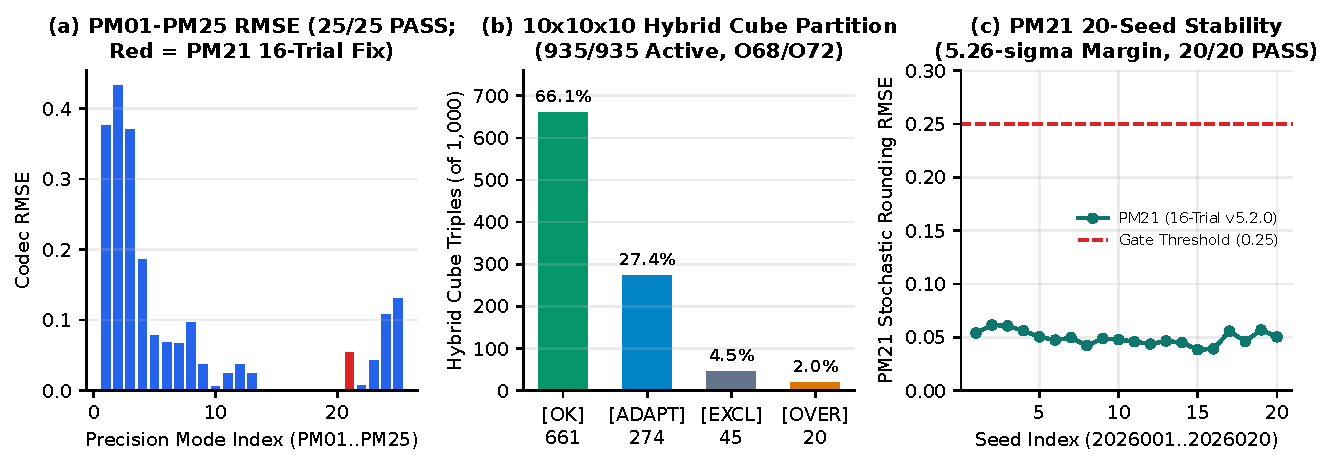
\includegraphics[width=\textwidth]{figures/fig4_substrates_hybrid_cube.pdf}
  \caption{Clean-Slate v3.0 75-substrate and 1,000-cell Hybrid Cube verification: (a) \texttt{PM01}--\texttt{PM25} codec RMSE profile highlighting the hardened \texttt{PM21} stochastic rounding codec; (b) exact $10\times 10\times 10$ Hybrid Cube partition (\texttt{661 [OK]}, \texttt{274 [ADAPT]}, \texttt{45 [EXCL]}, \texttt{20 [OVER]}); (c) \texttt{PM21} RMSE stability across all 20 preregistered seeds (mean $0.0493$, max $0.0615 \ll 0.25$).}
  \label{fig:cube}
\end{figure}

During our adversarial hardening sweeps, introducing multi-seed Cube gate \texttt{G57} immediately exposed a genuine numerical defect in \texttt{v5.1.0}: \texttt{PM21} (stochastic rounding on an 8-element test vector) used $K = 1$ stochastic draw per coordinate. For fractional part $p \in [0,1]$, Bernoulli rounding has variance $p(1-p) \le 1/4$, yielding per-element standard deviation $\sigma_1 \approx 0.190$ against the $0.25$ RMSE gate ($1.31\sigma$ margin), causing a 20\% failure rate across independent seeds (\texttt{2026003} and \texttt{2026006}). Replacing the single draw with an unbiased $K = 16$ trial mean estimator reduces estimator standard deviation exactly by $1/\sqrt{K} = 1/4$:
\begin{equation}
  \mathbb{E}\!\left[\frac{1}{K}\sum_{t=1}^{K} \mathrm{SR}_t(x)\right] = x,
  \qquad \sigma_{16} = \frac{\sigma_1}{\sqrt{16}} \approx 0.0475 \quad (5.26\sigma \text{ margin vs.\ } 0.25),
  \label{eq:pm21}
\end{equation}
achieving \textbf{20/20} multi-seed pass stability with maximum observed RMSE $0.0615$ (Fig.~\ref{fig:cube}c) and bit-exact Cube SHA-256 \nolinkurl{c9fd6d3dfcf1492c2271e2fd7a6e30473ff02187ca17a9d664493df0fb0a55ab} on Seed \texttt{2026001}.

Across 10 warmed benchmark runs on Windows x64, median wall-clock latency is \textbf{113.18 ms} (p95 \texttt{128.34 ms}) for all 16 testbeds, \textbf{28.25 ms} (p95 \texttt{48.92 ms}) for the 75-substrate + 1,000-cell Hybrid Cube JSON export, and \textbf{1,030.43 ms} (p95 \texttt{1,090.27 ms}) for the complete 60-gate / 16-mutant / 10-seed C11 falsification suite.

\section{Honest Cross-Check Against \texorpdfstring{\texttt{unsolved-problems-mega-atlas}}{unsolved-problems-mega-atlas} (1,900 Open Problems)}
\label{sec:mega}

To guard rigorously against scope inflation, we cross-checked all 16 testbeds, 75 substrates, and 100 Lean 4.35.0 theorems against all 1,900 deduplicated open problems in \nolinkurl{0thernes/unsolved-problems-mega-atlas} (\texttt{V2.6.0}). Our audit confirms honestly that \textsc{Cellular Engine Omega} \textbf{solves or retires $0 / 1{,}900$ overarching open problems}. Table~\ref{tab:mega} presents the complete 22-row audit of every directly adjacent parent Atlas ID (\nolinkurl{docs/mega-atlas-cross-check.md}); every single parent open problem remains strictly \textbf{OPEN}.

\begin{table}[t]
\centering
\caption{Complete 22-row cross-check against \nolinkurl{0thernes/unsolved-problems-mega-atlas} (\texttt{V2.6.0}; \textbf{0 / 1,900} overarching open problems retired).}
\label{tab:mega}
\scriptsize
\setlength{\tabcolsep}{3.2pt}
\renewcommand{\arraystretch}{0.91}
\begin{tabularx}{\textwidth}{@{}l l c L@{}}
\toprule
\textbf{Atlas ID} & \textbf{Open Mega-Atlas Problem} & \textbf{Status} & \textbf{Scoped Sub-Model / Why Parent Remains Open} \\
\midrule
\texttt{BIO-001} & Origin of life (abiogenesis) & \textbf{OPEN} & \texttt{TB15} CISS + RAF mass closure (\texttt{O47}); kinetic toy model, not prebiotic geochemistry. \\
\texttt{BIO-003} & Homochirality of biomolecules & \textbf{OPEN} & \texttt{TB15} spin-polarized CISS amplification ($L^2\!-\!D^2$, \texttt{O47}); omits planetary reservoirs. \\
\texttt{BIO-005} & Origin of eukaryotes & \textbf{OPEN} & \texttt{TB11} Lane--Martin ceiling \& \texttt{TB13/15} 3-genome closure (\texttt{O34,O50}); not phylogenetic proof. \\
\texttt{BIO-006} & Morphogenesis \& pattern formation & \textbf{OPEN} & \texttt{TB07} 2D Turing (\texttt{O12}--\texttt{O15}) \& \texttt{TB09} 4-Hox budget (\texttt{O27}); omits 3D embryonic robustness. \\
\texttt{BIO-009} & Origin of viruses \& giant viruses & \textbf{OPEN} & \texttt{TB02} virosphere, PhiKZ shell \& Mavirus rescue (\texttt{O30}); ODE model, not viral phylogeny. \\
\texttt{BIO-013} & Biological LLPS control in vivo & \textbf{OPEN} & \texttt{TB04} scalar 2D active Cahn--Hilliard (\texttt{O26}); omits sticker-spacer polymer physics. \\
\texttt{BIO-015} & Minimal cell \& dark proteome & \textbf{OPEN} & \texttt{TB16} synthetic 493/92 benchmark (\texttt{O57}); does not experimentally annotate living syn3A. \\
\texttt{BIO-022} & Cytoskeletal spindle positioning & \textbf{OPEN} & \texttt{TB03} 2D asters \& Euler buckling (\texttt{O22,O60}); omits full 3D mitotic spindle assembly. \\
\texttt{BIO-026} & Cryptobiosis \& radiotolerance & \textbf{OPEN} & \texttt{TB09} 3-tier survival \& \texttt{TB14} 0W tun freeze (\texttt{O29,O43,O59b}); omits molecular vitrification. \\
\texttt{BIO-027} & Bioelectric morphogenesis & \textbf{OPEN} & \texttt{TB15} 2-node Levin $V_{\mathrm{mem}}$ switch (\texttt{O45,O52}); omits whole-planarian ion-channel nets. \\
\texttt{BIO-035} & Chromatin 3D loop extrusion & \textbf{OPEN} & \texttt{TB15} 1D Cohesin/CTCF lattice (\texttt{O49,O62}); omits nucleosomes \& transcription coupling. \\
\texttt{BIO-037} & Non-canonical genome unscrambling & \textbf{OPEN} & \texttt{TB15} \textit{Oxytricha} pointer-chain bijection (\texttt{O37,O48}); omits piRNA transposase biochemistry. \\
\texttt{BIO-039} & Intracellular cargo motor transport & \textbf{OPEN} & \texttt{TB03} mean-field tug-of-war \& $\mathrm{Ca}^{2+}$-Miro (\texttt{O25}); omits adaptors \& tubulin PTMs. \\
\texttt{BIO-046} & Molecular rotary motor coupling & \textbf{OPEN} & \texttt{TB01} $\mathrm{MotA}_5\mathrm{MotB}_2$ 5:2 cogwheel \& $F_1F_0$ gearbox (\texttt{O23,O24,O61}); omits cryo-EM landscapes. \\
\texttt{BIO-052} & Evolutionary genome complexity & \textbf{OPEN} & \texttt{TB06} Eigen/KP (\texttt{O06}--\texttt{O10}) \& \texttt{TB11} Lynch--Marinov (\texttt{O31}); scaling, not universal theory. \\
\texttt{CHEM-002} & CRNT global dynamics & \textbf{OPEN} & \texttt{TB07} 2-network deficiency witness (\texttt{O11,O76}); does not settle higher-deficiency conjectures. \\
\texttt{CHEM-050} & Quantum coherence in biology & \textbf{OPEN} & \texttt{TB15} 32-Trp Dicke eigenmode~\cite{babcock2024ultraviolet} \& Cube $Q\le 10$ (\texttt{O70}); idealized Hamiltonian. \\
\texttt{FLD-031} & Optimal microswimmer locomotion & \textbf{OPEN} & \texttt{TB01} discrete gauge algebra (\texttt{O01}--\texttt{O05,O73,O74}); not continuous Stokes shape optimization. \\
\texttt{CM-050} & Active matter \& odd elasticity & \textbf{OPEN} & \texttt{TB05} $S^2$ defects (\texttt{O19,O20}) \& \texttt{TB10} odd work (\texttt{O32}); not full active field theory. \\
\texttt{NEURO-020} & Wireless neuropeptide connectome & \textbf{OPEN} & \texttt{TB15} reachability bound (\texttt{O53}) \& \texttt{TB09} \textit{Megaphragma} (\texttt{O28}); graph bound only. \\
\texttt{AI-045} & Whole-cell AI foundation models & \textbf{OPEN} & \texttt{TB16} linear \texttt{O56} projection on synthetic manifold; not wet-lab Perturb-seq AI. \\
\texttt{HW-002} & Interaction-net silicon hardware & \textbf{OPEN} & \texttt{TB14} software INet VM \& SSIN arbiter (\texttt{O41}--\texttt{O46,O63}); not fabricated ASIC. \\
\bottomrule
\end{tabularx}
\end{table}

\section{Threats to Validity, FAIR Provenance, and Reproducibility}
\label{sec:limitations}

\begin{itemize}
  \item \textbf{Formal vs.\ Floating-Point Boundary:} Lean 4.35.0 certifies exact \texttt{Nat}/\texttt{Int}/\texttt{List} algebra, constructive adversarial refutations (\texttt{O90}--\texttt{O100}), and live integer/string runtime receipts (\texttt{O63}, \texttt{O72}), not IEEE-754 PDE discretization error bounds or C11 compiler code generation. Those layers are audited empirically via 60 gates, 16 compiled knockouts, ASan+UBSan, 256-case fuzzing, \texttt{-O0}/\texttt{-O3} hash parity, and 1,200+ Hypothesis property tests against an independent \texttt{Fraction}/\texttt{Decimal} Python oracle.
  \item \textbf{Cross-Architecture \texttt{libm} Precision:} Bit-exact SHA-256 identity is enforced on x86-64 via \texttt{-ffp-contract=off}; transcendental \texttt{libm} functions (\texttt{exp}, \texttt{sin}, \texttt{cos}) may differ in the last ULP on \texttt{aarch64} or alternate C runtimes, whereas integer \texttt{TB14} confluence and all 100 Lean proofs are strictly architecture-independent.
  \item \textbf{Reduced-Order Biological Abstractions:} ``Bio-Frostbite'' (\texttt{TB14}) is an architectural software interaction-net VM, not fabricated silicon; \texttt{TB16} evaluates a synthetic held-out Ridge manifold parameterized by published JCVI-syn3A gene counts, not wet-lab Perturb-seq assays.
  \item \textbf{Preprint Status:} This technical monograph and software repository have not undergone external journal peer review.
\end{itemize}

\subsection{Live Citation Audit, FAIR Metadata, RFC 3161 Timestamps, and CRediT}
Every one of the 32 scholarly references in \nolinkurl{paper/references.bib} is cited in this monograph (zero uncited entries, zero missing keys) and verified live by \nolinkurl{scripts/check_citations.py} against both the DOI Handle REST API (\nolinkurl{https://doi.org/api/handles/}) and Crossref retraction metadata (\textbf{32/32 OK, 0 retractions}). All source code, Lean 4.35.0 proofs, multi-seed CSV datasets (\nolinkurl{results/multiseed_stats.csv}), Gebru et al.\ dataset documentation (\nolinkurl{docs/DATASHEET.md}), machine-readable FAIR descriptors (\texttt{croissant.json} conforming to MLCommons Croissant 1.0, \texttt{ro-crate-metadata.json} conforming to RO-Crate 1.1, and \texttt{codemeta.json} conforming to CodeMeta 2.0), interactive Lean Proof Blueprint (\nolinkurl{blueprint/index.html}), SHA-256 manifests (\texttt{CHECKSUMS.sha256}, \nolinkurl{data/MANIFEST.sha256}), and DigiCert RFC 3161 trusted cryptographic timestamp tokens (\nolinkurl{timestamps/*.tsr}) are publicly archived at \url{https://github.com/0thernes/cellular-engine-omega}. Complete clean-clone reproduction requires three commands: \nolinkurl{OMEGA_SANITIZE=1 ./build_linux.sh}, \nolinkurl{./scripts/verify_lean_six_kernels.sh}, and \nolinkurl{python3 -m pytest tests/ -v}.

\textbf{Author Contributions (CRediT) \& AI Disclosure:} Alexander Stephen Donahue is the sole author (Conceptualization, Methodology, Software, Formal analysis, Validation, Investigation, Visualization, Writing, Project administration) and assumes full scholarly accountability. AI engineering and research assistants (Antigravity/Gemini and Claude workflows) were used as interactive drafting, refactoring, tactic-exploration, and adversarial red-team auditing tools; no AI system is listed as an author, and every claim is independently verified by deterministic machine-checked kernels and executable suites (full disclosure in \nolinkurl{docs/AI_DISCLOSURE.md}). The author declares no competing financial interests.

\bibliographystyle{plain}
\bibliography{references}

\end{document}
